\vspace{-0.2cm}
\subsection{Memorizing Atypical Samples Hurts Typical Samples' Performance}\label{sec:pre2}
\vspace{-0.2cm}

%\jt{for Figure 2, Because of the high performance of clean performance, currently the difference of adversarial performance with different portions of atypical examples is not such obvious. can we put all adversarial performance in one figure and the clean performance in the other? In this way, I think the difference will be much more obvious}

In this subsection, we further observe that fitting atypical samples will even bring negative effects on ``typical'' samples. Here, we define ``typical'' samples as the subset of training set $\mathcal{D}$ which have low memorization value: $\mathcal{D}_\text{typ} = \{x_i\in\mathcal{D}:\text{mem}(x_i)<0.02\}$. It means that they are not fitted by memorization and are from the main sub-population in their class. To define the test typical set $\mathcal{D}'_\text{typ}$, we exclude all test samples which have high influence values from any atypical training samples, and also exclude the samples that using ERM algorithm $\mathcal{A}$ has low success rate to predict (the samples which cannot be learned from $\mathcal{D}$): $\mathcal{D}'_\text{typ} = \mathcal{D}' - \{x'_j: \text{infl}(x_i,x'_j)> 0.02, \text{for } \forall x_i\in \mathcal{D}_\text{atyp}\} \cup \{x'_j: \text{Pr.}_{F\leftarrow\mathcal{A}(\mathcal{D})}(F(x'_j) = y_j) < 0.8\}$.

\begin{figure}[t]
\centering
\hspace*{-1cm}
\subfloat[Clean (left) \& Adv Acc. (right) under ResNet18.]{
\label{fig:hurt1}
\begin{minipage}[c]{0.55\textwidth}
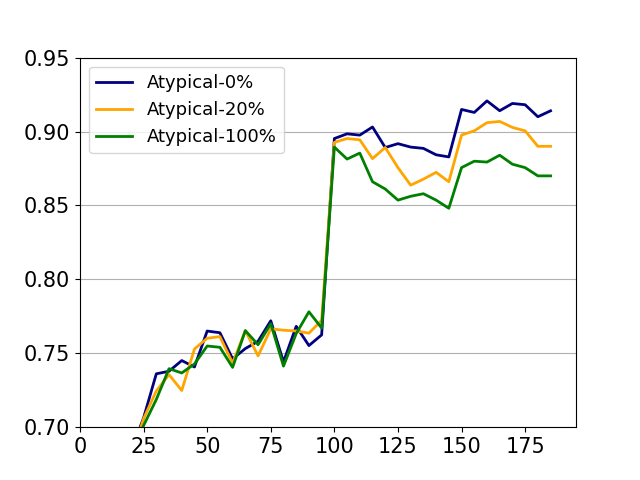
\includegraphics[width = 0.5\textwidth]{figures/poison_clean_ResNet18.png}%
\hfill
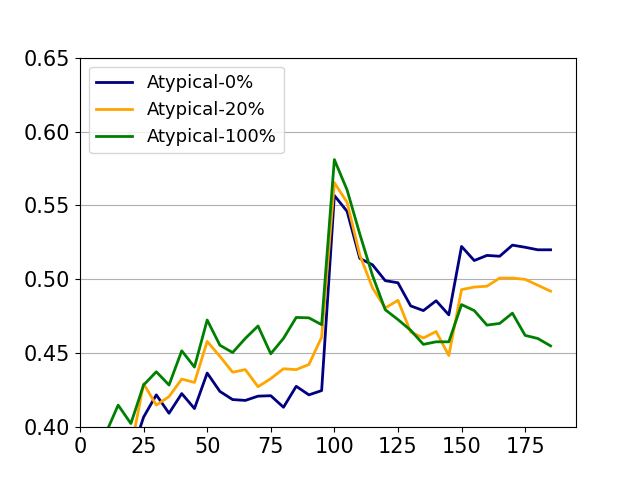
\includegraphics[width = 0.5\textwidth]{figures/poison_adv_ResNet18.png}
\end{minipage}
}
\hspace*{-0.4cm}
\subfloat[Clean (left) \& Adv Acc. (right) under WRN28.]{
\label{fig:hurt2}
\begin{minipage}[c]{0.55\textwidth}
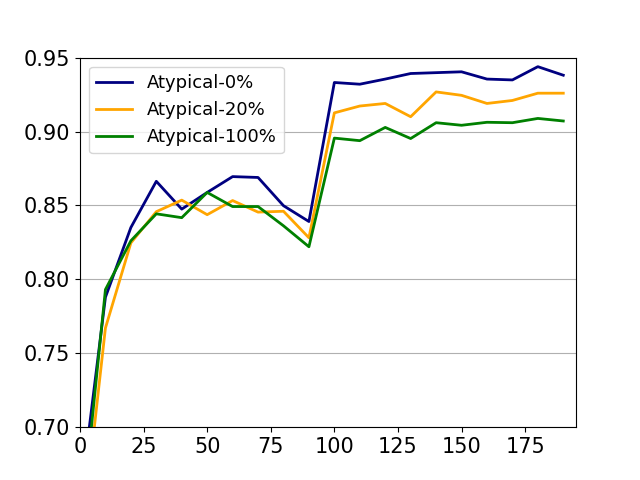
\includegraphics[width = 0.5\textwidth]{figures/poison_clean_WRN.png}%
\hfill
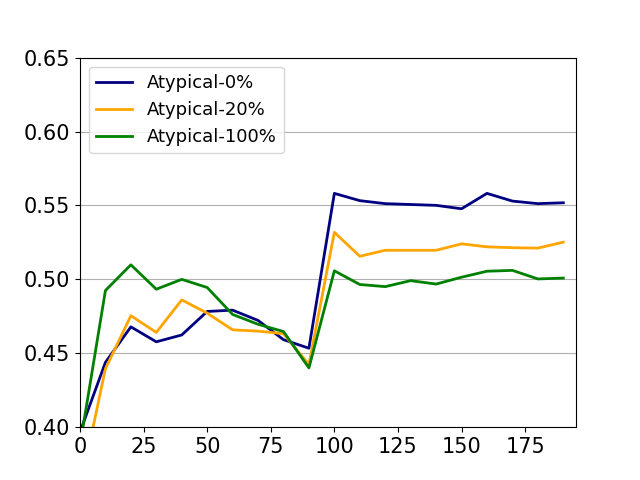
\includegraphics[width = 0.5\textwidth]{figures/poison_adv_WRN.png}
\end{minipage}
}
\caption{Clean Accuracy and Adversarial Accuracy on \textbf{Typical} Set of CIFAR100}
\vspace{-0.5cm}
\label{fig:hurt}
\end{figure}
To demonstrate the negative effect from fitting atypical samples, we conduct PGD adversarial training~\cite{madry2017towards} for several trails on resampled CIFAR100 datasets: each dataset is constructed with the whole training typical set $\mathcal{D}_\text{typ}$, and a part of the training atypical set $\mathcal{D}_\text{atyp}$ (randomly sample 0\%, 20\% and 100\% in $\mathcal{D}_\text{atyp}$). In Fig.~\ref{fig:hurt}, we report the adversarially trained model's clean and adversarial accuracy on the test typical set $\mathcal{D}_\text{typ}'$ and check the impact of atypical samples on the typical samples. From the results, we find that the amount of atypical samples makes a significant influence on the typical samples. For example, under ResNet18, an adversarially trained model without atypical samples has 92\% clean accuracy and 52\% adversarial accuracy on the test typical samples (on the last epochs). While, the model trained with all atypical samples included only has 85\% and 44\% clean \& adv. accuracy, respectively. 
These results suggest: the more atypical samples exist in training set, the poorer performance the model will have on $\mathcal{D}'_\text{typ}$. In other words, these atypical samples act more like ``poisoning'' samples~\cite{biggio2012poisoning, xu2019adversarial} which can deteriorate the model's performance on typical samples and consequently hurt the overall performance. 


\noindent\textbf{Poisoning Atypical Samples} A natural question is what kind of atypical samples are likely to ``poison'' model robustness and why? Different from previous literature about poisoning samples in traditional ERM, which assume that poisoning samples are most mis-labeled samples~\cite{li2020gradient}, CIFAR100 is a clean dataset with no or very few wrong labels. However, we hypothesize that the atypical samples which poison the model performance might pertain some features of a ``wrong'' class. Recall that atypical samples are always distinct from the main data distribution in their labeled class, it is likely that they are closer to the distribution of a ``wrong'' class. As shown in  Fig.~\ref{fig:atypical_samples}, an atypical ``plate'' is visually very similar to images in ``apple''. If the model memorizes this atypical ``plate'' and predicts any samples with similar features to be ``plate'', the model cannot distinguish between ``apple'' and ``plate''. As a simple verification to this hypothesis, in Table~\ref{Tab:dist}, we empirically show that atypical samples can cause adversarial training to produce ``less-discriminative'' representations among different classes. Under the same experimental setting and the models above, we measure the average \textit{Cosine Distance (CD)~\footnotemark} of the models' pen-ultimate layer representation output, for each pair of samples (in the training typical set $\mathcal{D}_\text{typ}$) from different classes. Table~\ref{Tab:dist} shows that in adversarial training, fitting more atypical samples will result in a smaller distance for the representations of samples in different classes. It suggests that with atypical samples, DNNs learn more similar and mixed representations for different classes, which can degrade the typical samples' test performance.
\begin{table}[h]
\vspace{-0.5cm}
\small
\centering
\setlength{\tabcolsep}{12pt}
\caption{Class-wise Cosine Distance of Representations of Typical Samples}
\begin{tabular}{c|ccc}
\hline
\# of Atypical Samples & 0\% &20\% &100\%\\
\hline
ResNet18 & 0.66 & 0.62  & 0.59\\
\hline
WRN28 &0.64 & 0.61 & 0.57\\
\hline
\end{tabular}
\vspace{-0.4cm}
\label{Tab:dist}
\end{table}

\footnotetext{Cosine Distance: $\E_{x_1,x_2} [\frac{h(x_1)\cdot h(x_2)}{||h(x_1)||_2\cdot||h(x_2)||_2}]$, where $h(\cdot)$ is the pen-ultimate layer output of DNN model $F(\cdot)$, and $x_1,  x_2\in \mathcal{D}_\text{typ}$ and from different classes.}


It is also worth to mention that this poisoning phenomenon does not appear in the traditional ERM algorithm (results in Appendix~\ref{app:pre}). In ERM, memorizing atypical samples will neither hurt typical sample's performance or degrade the feature space discrimination. A possible explanation is that adversarially trained models use more ``semantically meaningful'' features for prediction~\cite{tsipras2018robustness, ilyas2019adversarial}. During adversarial training, the models will not only memorize the labels of atypical samples, but also their semantic features. As a result, the adversarial trained DNNs will construct more mixed concepts of features, if the ``poisoning'' atypical samples exist.


\begin{figure}[t]
\subfloat{
\label{fig:poison_pair1}
\begin{minipage}[c]{0.5\textwidth}
\centering
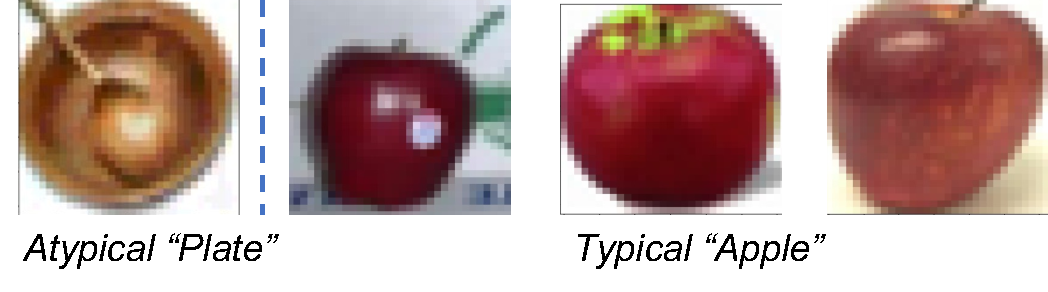
\includegraphics[width = 0.8\textwidth]{figures/poison_pair1.pdf}
\end{minipage}
}
\subfloat{\label{fig:poison_pair2}
\begin{minipage}[c]{0.5\textwidth}
\centering
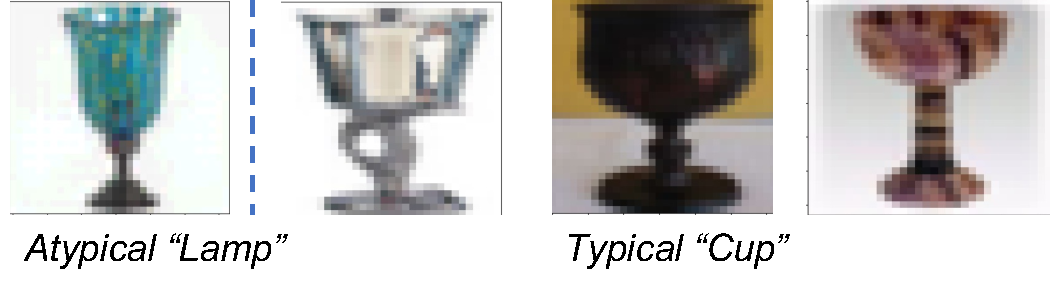
\includegraphics[width = 0.8\textwidth]{figures/poison_pair2.pdf}
\end{minipage}
}
\caption{Examples of Poisoning Atypical Samples}
\vspace{-0.4cm}
\label{fig:atypical_samples}
\end{figure}